\documentclass{beamer}
\usepackage{tikz,amsmath,hyperref,graphicx,stackrel}
\usetikzlibrary{positioning,shadows,arrows,shapes,calc}
\newcommand{\argmax}{\operatornamewithlimits{argmax}}
\newcommand{\argmin}{\operatornamewithlimits{argmin}}
\mode<presentation>{\usetheme{Frankfurt}}
\AtBeginSection[]
{
  \begin{frame}<beamer>
    \frametitle{Outline}
    \tableofcontents[currentsection,currentsubsection]
  \end{frame}
}
\title{Lecture 1: Review of Calculus and Complex Numbers}
\author{Mark Hasegawa-Johnson}
\date{ECE 401: Signal and Image Analysis, Fall 2020}  
\begin{document}

% Title
\begin{frame}
  \maketitle
\end{frame}

% Title
\begin{frame}
  \tableofcontents
\end{frame}

%%%%%%%%%%%%%%%%%%%%%%%%%%%%%%%%%%%%%%%%%%%%
\section[Outline]{Outline of today's lecture}
\setcounter{subsection}{1}
\begin{frame}
  \frametitle{Outline of today's lecture}
  \begin{enumerate}
  \item \href{https://courses.engr.illinois.edu/ece401/fa2020/\#syllabus}{\bf\color{blue}Syllabus}
  \item \href{https://courses.engr.illinois.edu/ece401/fa2020/hw1.pdf}{\bf\color{blue}Homework 1}
  \item \href{https://www.pearson.com/us/higher-education/program/Mc-Clellan-DSP-First-2nd-Edition/PGM86857.html}{\bf\color{blue}Textbook}
  \item Review: Integration, Summation, and Complex numbers
  \end{enumerate}
\end{frame}

%%%%%%%%%%%%%%%%%%%%%%%%%%%%%%%%%%%%%%%%%%%%
\section[Integration]{Review: How to integrate an exponential}
\setcounter{subsection}{1}

\begin{frame}
  \frametitle{Integration = Computing the area under a  curve}
  \centerline{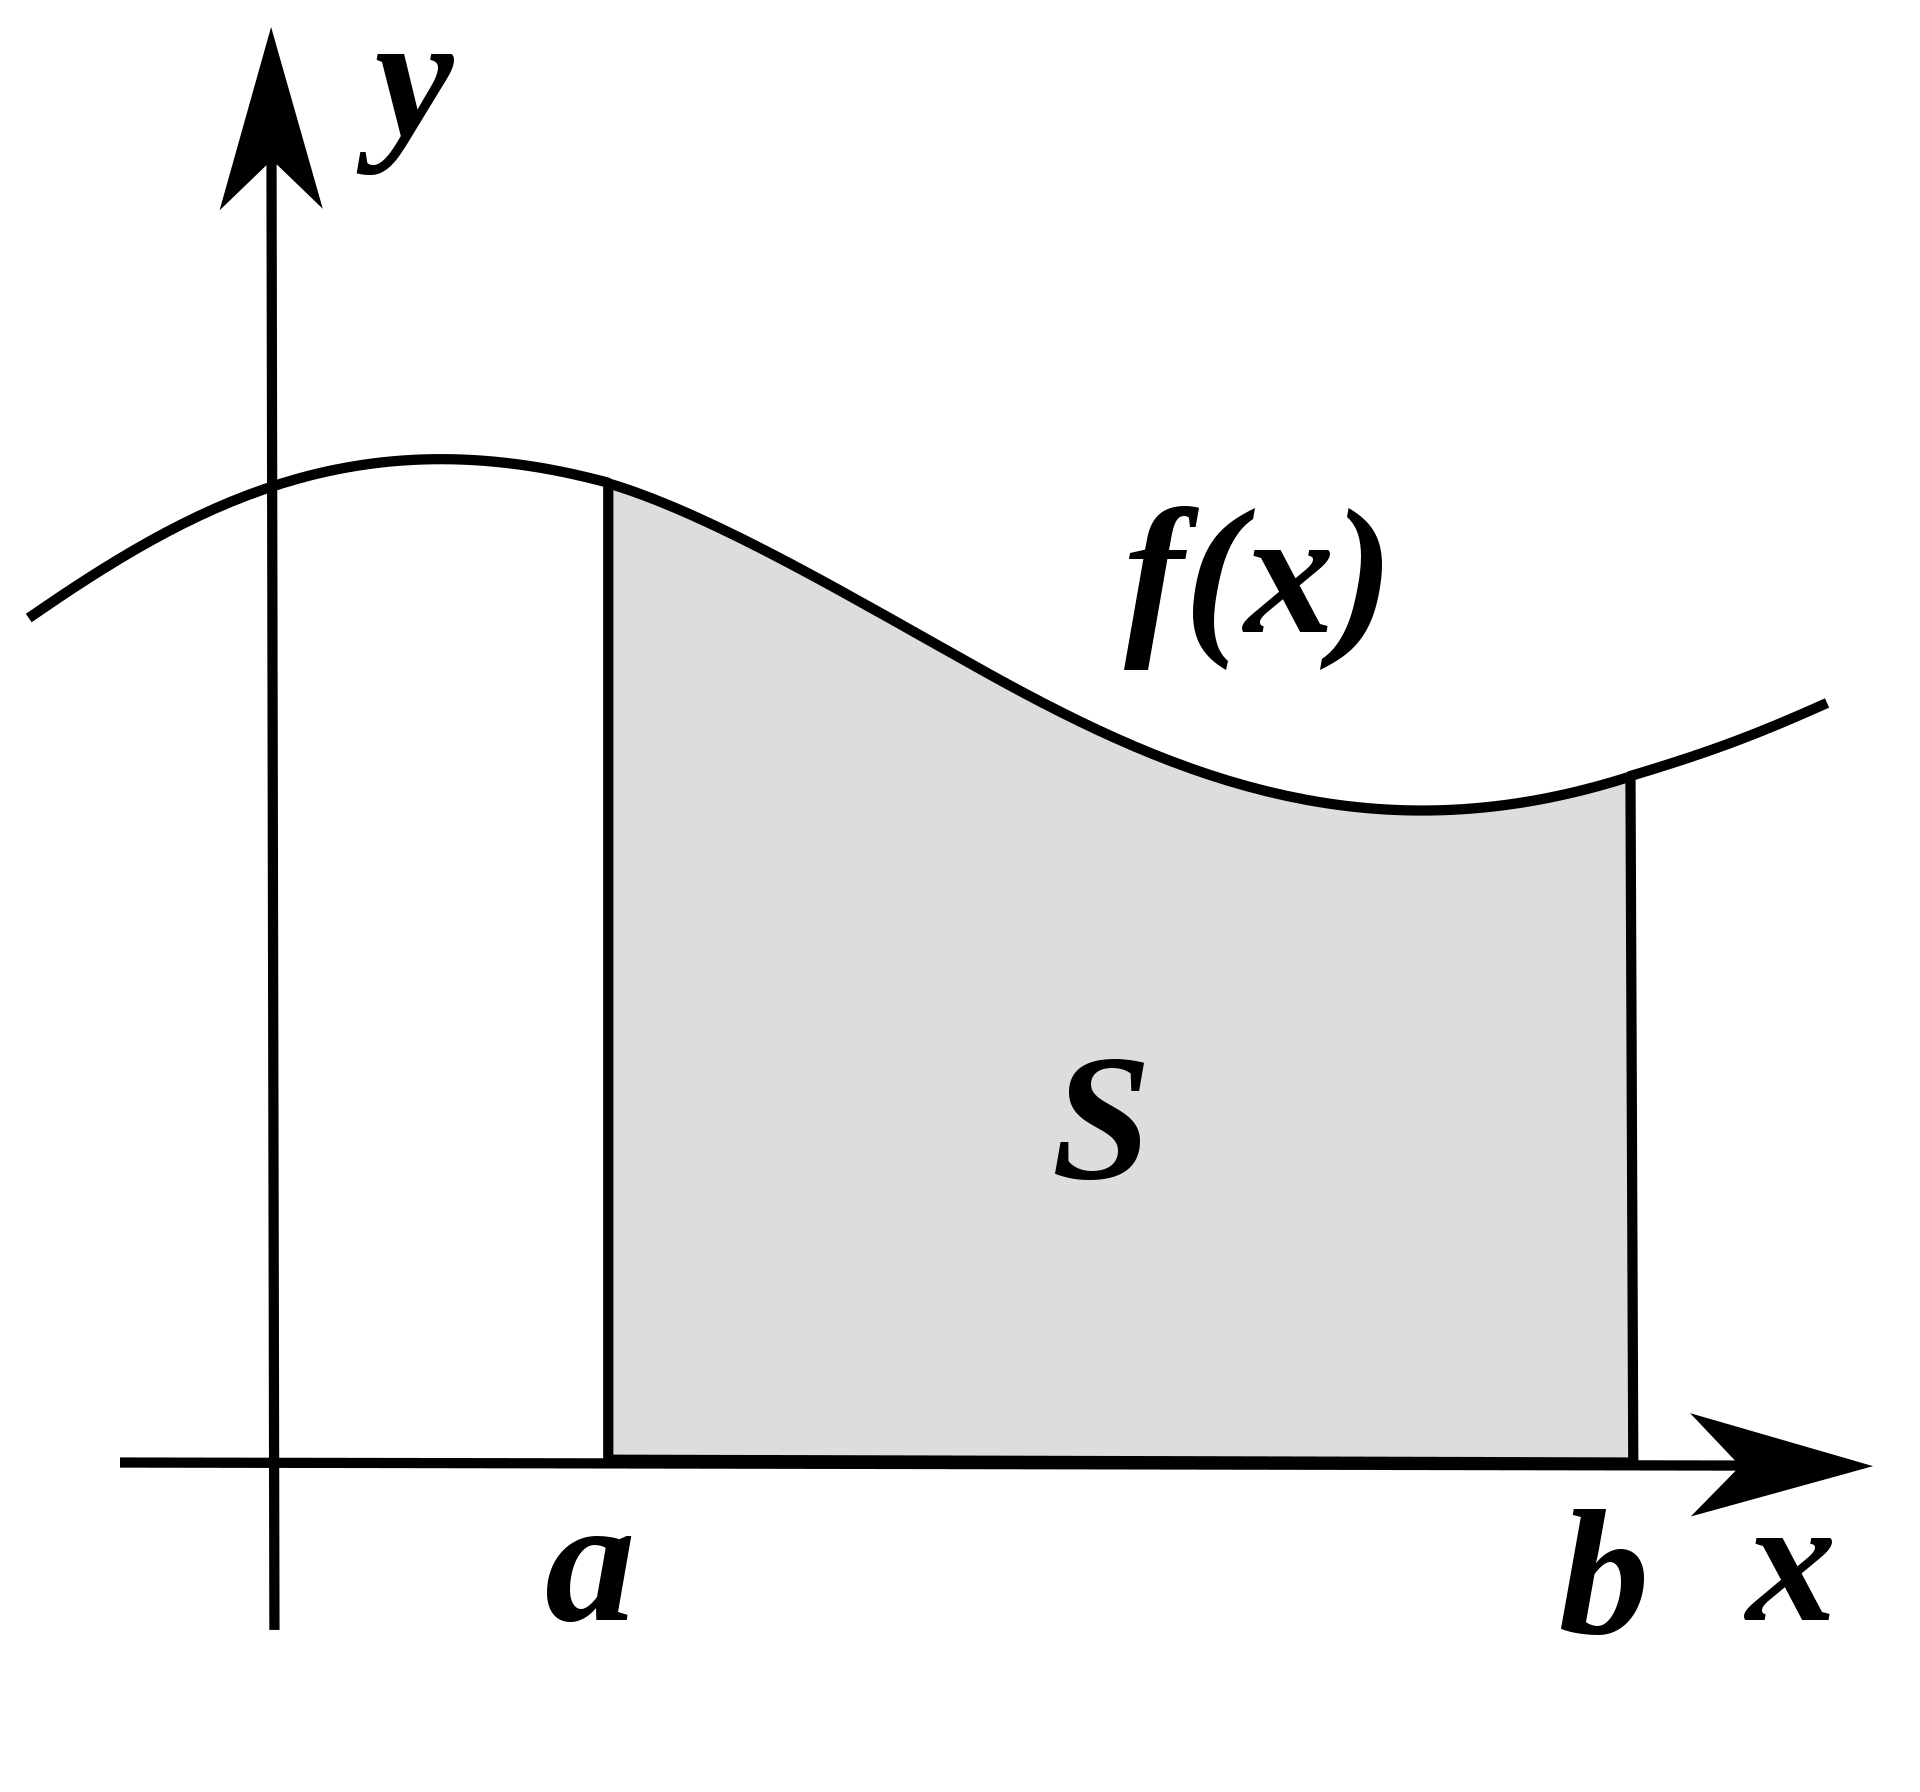
\includegraphics[height=2in]{fig1.png}}
  \begin{tiny}
    Gnu Free Documentation License, By 4C,
    \url{https://commons.wikimedia.org/wiki/File:Integral_as_region_under_curve.svg}
  \end{tiny}
\end{frame}

\begin{frame}
  \frametitle{Why does signal processing use integrals?}
  \begin{itemize}
  \item Real-world {\bf signals} are functions of continuous time, or space,
    or both.  For example, sound is air pressure as a function of
    time, $p(t)$.
  \item The {\bf energy} necessary to produce a signal depends on its
    long-term integral:
    \[
    E \propto \int_{-\infty}^\infty p^2(t)dt
    \]
  \item The {\bf information} in a signal is encoded at different
    frequencies ($f$), which we can get using something called a {\bf
      Fourier transform}.  For continuous-time signals, a Fourier
    transform is an integral:
    \[
    P(f) = \int_{-\infty}^\infty p(t)e^{-j2\pi f t}dt
    \]
  \end{itemize}
\end{frame}
    
\begin{frame}
  \frametitle{Indefinite vs. definite integrals}
  \begin{itemize}
  \item An {\bf indefinite integral} (a.k.a. antiderivative) is the opposite
    of a derivative:
    \[
    F(x) = \int f(x) ~~~\mbox{means that}~~~ f(x) = \frac{dF}{dx}
    \]
  \item A {\bf definite integral} is the area under the curve.  We can write it as:
    \[
    \int_a^b f(x)dx = \left[F(x)\right]_a^b = F(b)-F(a)
    \]
  \end{itemize}
\end{frame}

\begin{frame}
  \frametitle{Indefinite integrals worth knowing}
  \begin{itemize}
  \item Integral of a polynomial:
    \[
    \int x^n dx = \frac{1}{n+1} x^{n+1}
    \]
  \item Integral of an exponential:
    \[
    \int e^{x} dx = e^{x}
    \]
  \end{itemize}
\end{frame}

\begin{frame}
  \frametitle{Methods for turning one integral into another}
  \begin{itemize}
  \item Variable substitution: Suppose $f(x)=g(u)$ where $u$ is some
    function of $x$.  There is no other $x$ anywhere inside $f(x)$.  Then:
    \[
    \int g(u)dx = \int \frac{1}{du/dx}g(u)du
    \]
  \item
    Integration by parts:
    \[
    \int u dv = uv - \int v du
    \]
  \end{itemize}
\end{frame}

\begin{frame}
  \frametitle{Example: How to integrate an exponential}
  \centerline{\fbox{What is $\int_{0.4}^{1.6} e^{j((x+y)t+\theta)} dt$?}}
  \begin{enumerate}
    \item Pull out the constants:
      \[
      \int_{0.4}^{1.6} e^{j((x+y)t+\theta)} dt = e^{j\theta}\int_{0.4}^{1.6} e^{j(x+y)t} dt
      \]
    \item Prepare for variable substitution:
      \begin{align*}
        u = j(x+y)t &~~~\mbox{means that}~~~ \frac{du}{dt} = j(x+y)\\
        t\in[0.4,1.6] &~~~\mbox{means that}~~~ u\in [j(x+y)0.4,j(x+y)1.6]
      \end{align*}
    \item Variable substitution:
      \[
      \int_{0.4}^{1.6} e^{j(x+y)t} dt=\int_{j(x+y)0.4}^{j(x+y)1.6} \frac{1}{j(x+y)}e^{u} du
      \]
  \end{enumerate}
\end{frame}
\begin{frame}
  \frametitle{Example: How to integrate an exponential}
  \begin{enumerate}
    \setcounter{enumi}{3}
  \item Pull out the constants again:
    \[
    \int_{j(x+y)0.4}^{j(x+y)1.6} \frac{1}{j(x+y)}e^{u} du =
    \frac{1}{j(x+y)}  \int_{j(x+y)0.4}^{j(x+y)1.6} e^{u} du
    \]
  \item Integrate:
    \[
    \int_{j(x+y)0.4}^{j(x+y)1.6} e^{u} du=
    \left[e^u\right]_{j(x+y)0.4}^{j(x+y)1.6}
    \]
  \item Solve:
    \[
    \int_{0.4}^{1.6} e^{j((x+y)t+\theta)} dt =
    \frac{e^{j\theta}}{j(x+y)}\left(e^{j(x+y)1.6}-e^{j(x+y)0.4}\right)
    \]
  \end{enumerate}
\end{frame}

%%%%%%%%%%%%%%%%%%%%%%%%%%%%%%%%%%%%%%%%%%%%
\section[Summation]{Review: Summing a geometric series}
\setcounter{subsection}{1}

\begin{frame}
  \frametitle{Summation is a computer-friendly version of integration}
  \centerline{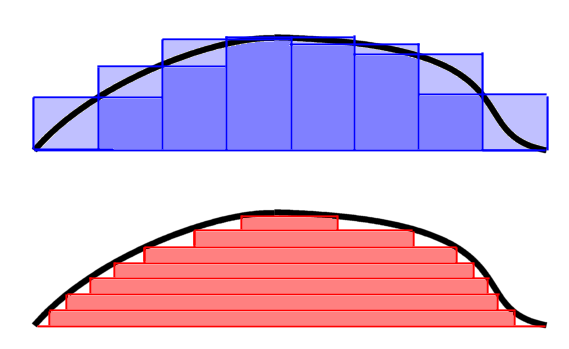
\includegraphics[height=2in]{fig2.png}}
  \begin{tiny}
  Author unknown, GFDL,
  \url{https://commons.wikimedia.org/wiki/File:RandLintegrals.png}
  \end{tiny}
\end{frame}

\begin{frame}
  \frametitle{Why does signal processing use sums?}
  \begin{itemize}
  \item On computers, a signal is a sequence of numbers $x[n]$,
    regularly spaced samples of some real-world signal.
  \item The {\bf energy} necessary to produce a signal depends on its
    long-term summation
    \[
    E \propto \sum_{-\infty}^\infty x^2[n]
    \]
  \item The {\bf information} in a signal is encoded at different
    frequencies ($f$), which we can get using something called a {\bf
      Fourier transform}.  For discrete-time signals, a Fourier
    transform is a summation
    \[
    X(\omega) = \sum_{-\infty}^\infty x[n] e^{-j\omega n}
    \]
  \end{itemize}
\end{frame}

\begin{frame}
  \frametitle{Sums worth knowing}
  \begin{itemize}
  \item Exponential series:
    \[
    \sum_{n=0}^\infty \frac{1}{n!} x^n = e^x
    \]
  \item Geometric series:
    \[
    \sum_{n=0}^{N-1} r^n = \frac{1-r^N}{1-r}
    \]
  \end{itemize}
\end{frame}

\begin{frame}
  \frametitle{Example: How to sum a geometric series}
  \centerline{\fbox{Problem: What is $\sum_{n=-7}^7 e^{-j\omega n}$?}}
  \begin{enumerate}
  \item Prepare for variable substitution \#1:
    \begin{align*}
      m=n+7 &~~~\mbox{means that}~~~ n=m-7 \\
      n\in [-7,7] &~~~\mbox{means that}~~~ m\in [0,14]
    \end{align*}
  \item Variable substitution \#1:
    \[
    \sum_{n=-7}^7 e^{-j\omega n} =\sum_{m=0}^{14} e^{-j\omega (m-7)}
    \]
  \item Pull out the constants:
    \[
    \sum_{m=0}^{14} e^{-j\omega (m-7)} =e^{7j\omega}\sum_{m=0}^{14}e^{-j\omega m}
    \]
  \end{enumerate}
\end{frame}
\begin{frame}
  \frametitle{Example: How to sum a geometric series}
  \begin{enumerate}
    \setcounter{enumi}{3}
  \item Prepare for variable substitution \#2:
    \[
    r=e^{-j\omega} ~~~\mbox{means that}~~~  e^{-j\omega m}=r^m
    \]
  \item Variable substitution \#2:
    \[
    e^{7j\omega}\sum_{m=0}^{14}e^{-j\omega m} = e^{7j\omega}\sum_{m=0}^{14}r^m
    \]
  \item Sum:
    \[
    \sum_{m=0}^{14}r^m=\frac{1-r^{15}}{1-r}
    \]
  \item Solve:
    \[
    \sum_{n=-7}^7 e^{-j\omega n} = e^{7j\omega}\left(\frac{1-e^{-j15\omega}}{1-e^{-j\omega}}\right)
    \]
  \end{enumerate}
\end{frame}

%%%%%%%%%%%%%%%%%%%%%%%%%%%%%%%%%%%%%%%%%%%%
\section[Complex Numbers]{Review: Complex numbers}
\setcounter{subsection}{1}

\begin{frame}
  \frametitle{Complex numbers}
  \centerline{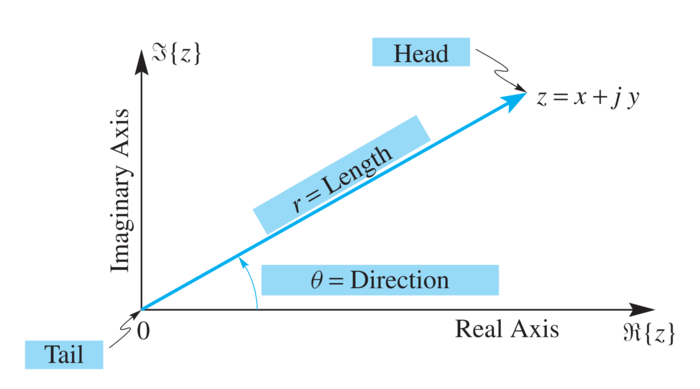
\includegraphics[height=2in]{fig3.png}}
  \begin{tiny}
    Copyright 2016, Pearson Education, Inc.
  \end{tiny}
\end{frame}

\begin{frame}
  \frametitle{Why does signal processing use complex numbers?}
  \begin{itemize}
  \item The Fourier transform was originally defined in terms of cosines and sines:
    \[
    X(\omega,\theta) = \int_{-\infty}^\infty x(t) \cos(\omega t+\theta)dt
    \]
  \item \ldots but exponentials are easier to integrate than cosines, and {\bf a lot} easier to
    sum.
  \item \ldots so we take advantage of Euler's equation, to turn all of the
    cosines and sines into exponentials:
    \[
    e^{j\omega t} = \cos(\omega t) + j\sin(\omega t)
    \]
  \end{itemize}
\end{frame}

\begin{frame}
  \frametitle{Rectangular and polar coordinates}
  \[
  z = x+jy = me^{j\theta}
  \]
  \begin{itemize}
  \item Converting rectangular to polar coordinates:
    \[
    m = \sqrt{x^2+y^2},~~~
    \theta =
    \begin{cases}
      \mbox{atan}\left(\frac{y}{x}\right) & x>0\\
      \pm \frac{\pi}{2} & x=0\\
      \mbox{atan}\left(\frac{y}{x}\right) \pm\pi & x<0
    \end{cases}
    \]
  \item Converting polar to rectangular:
    \[
    x=m\cos\theta,~~~y=m\sin\theta
    \]
  \end{itemize}
\end{frame}

\section{Summary}
\begin{frame}
  \frametitle{Summary}
  \begin{enumerate}
  \item Integration:
    \[
    \int e^xdx = e^x,~~~~\int g(u)dx=\int\frac{1}{du/dx}g(u)du
    \]
  \item Summation
    \[
    \sum_{n=0}^{N-1} r^n = \frac{1-r^N}{1-r}
    \]
  \item Complex numbers:
    \[
    m = \sqrt{x^2+y^2},~~~
    \theta =
    \begin{cases}
      \mbox{atan}\left(\frac{y}{x}\right) & x>0\\
      \pm \frac{\pi}{2} & x=0\\
      \mbox{atan}\left(\frac{y}{x}\right) \pm\pi & x<0
    \end{cases}
    \]
  \end{enumerate}
\end{frame}
\end{document}

